\section{NMOS threshold}\label{nmos_dimensioning}
First we take a look at the pull down network, which is being formed by the NMOS transistors.
We have to make sure that the pull down network will effectively tie our output signal to ground, latest when reaching the voltage defined as high signal (inverter!)

As shown in  \autoref{TTL_logic_levels} our acceptable voltages for our CMOS "ON" state range from 0V to 2V

\begin{figure}[H]
	\centering
	\begin{circuitdiagram}{20}{20}
		\power{15}{18.5}{U}{}  % power above resistor
		\wire{15}{17}{15}{18}   % wire above resistor
		\resis{15}{14}{V}{$R_D$}{}  % resistor on drain
		\wire{15}{11}{15}{8}   % wire between resistor and nmos
		\trans{nenh}{13}{6}{R}{}{} % nmos -> right
		\Voltarrow{10}{4}{14}{1}{d}{$+V_{GS}$}
		\wire{15}{1}{15}{4}   % wire below nmos
		\ground{15}{0.5}{D}  % ground below nmos
		\othersrc[\sigsym{rec}]{o}{5.5}{4.5}{H}{}{signal}
		\pin{9.5}{4.5}{R}{}	% pin in
		\ground{2.5}{0.5}{D}  % ground below signal source
		\wire{2.5}{1}{2.5}{4.5}   % wire below signal
		\junct{15}{10}   % dot
		\wire{15}{10}{16}{10}   % wire before out
		\pin{17}{10}{R}{out}	% pin out
	\end{circuitdiagram}
	\caption{enhancement-mode NMOS transistor use-case}
\end{figure}

\begin{equation}
V_{off} \leq 0.8 V
\end{equation}

With the values derived from \autoref{gate_dimensioning} which gives us the thickness of the gate ($\approx 40nm$) we target a threshold voltage of $0.8V$,  so that we switch the pull down circuit as soon as the low-signal is on.

We target a concentration of $N_p = 10^{16}\frac{1}{cm^3}=10^{22}\frac{1}{m^3}$.

The depletion zone thickness at its peak will be $W_{dmax} \approx 2.73 \cdot 10^{-7} m = 273 nm$

With an implantation (or constant source diffusion step), we can now set a range/energy and dosage in order to cover the depletion zone area.

For getting the energy and dose we look at \autoref{graphics_range_and_straggle} or use the web tool linked in the implant chapter.

The depth of the p-well $\approx 2 \mu m$ comes mainly from the need to fulfill the condition from \autoref{physics_drive_in}

\begin{equation}
x_e = 2 \cdot \sqrt{D_e \cdot t_e} \gg 2 \cdot \sqrt{D_v \cdot t_v} = x_v
\end{equation}

\newpage

We already got the background ($N_B \approx 7 \cdot 10^{14} \frac{1}{cm^3}=7 \cdot 10^{20} \frac{1}{m^3}$) concentration from the specs of the basis substrate.

\begin{equation}
N_p - N_B = 10^{22}\frac{1}{m^3} - 7 \cdot 10^{20} \frac{1}{m^3} = 9.3 \cdot 10^{21} \frac{1}{m^3}
\end{equation}

We use a drive in temperature of $1150 \degree C$ which is  $T = 1423.15 \degree K$ in Kelvin which gives us the diffusion coefficient $D=9.1 \cdot 10^{-17}  \frac{m^2}{s}$

Now using
\begin{equation}
N(x,t)
=
\frac{Q}{\sqrt{\pi\cdot D \cdot t}} \cdot \exp\left(\frac{-x^2}{4 \cdot D \cdot t}\right)
\end{equation}

We set the conditions and get the required diffusion time as well as the initial dosage in one shot:
\begin{equation}
N(0,t)
=
\frac{Q}{\sqrt{\pi\cdot D \cdot t}}
=
N_p-N_B
=
7 \cdot 10^{20} \frac{1}{m^3}
\end{equation}
\begin{equation}
x
=
2 \cdot \sqrt{D \cdot t \cdot\ln\left(\frac{N_T}{N_B}\right)}
=
2 \mu m
=
2 \cdot 10^{-6} m
\end{equation}
\begin{equation}
\Rightarrow
t \approx 4259s \approx \underline{70 min}
\end{equation}
\begin{equation}
\Rightarrow
Q
=
7 \cdot 10^{20} \frac{1}{m^3} \cdot \sqrt{\pi\cdot D \cdot t}
\approx
\underline{1.02 \cdot 10^{16} \frac{1}{m^2}}
\end{equation}

If we plot the functions from our calculation we can yield the below graphics\footnote{see simulation/diffusion\_pwell.wxmx}

\begin{figure}[H]
	\centering
	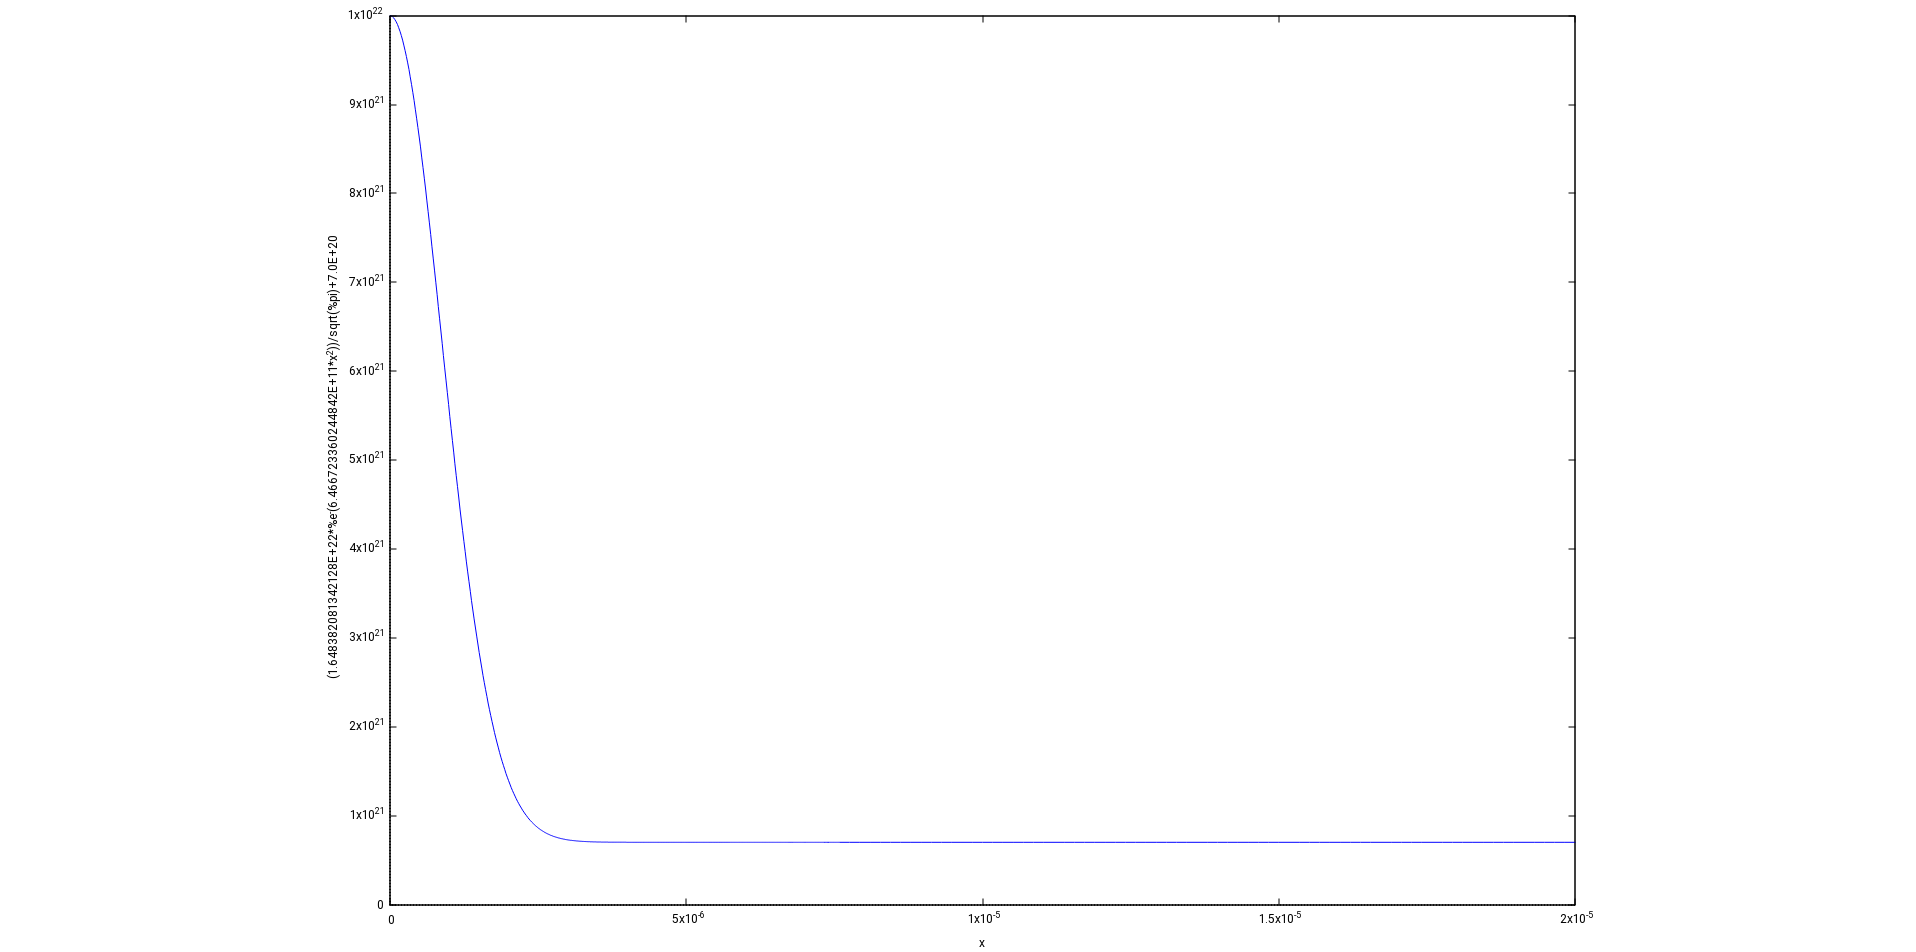
\includegraphics[width=0.75\textwidth]{p-well-diffusion.png}
	\caption{Dopant concentration after around 70 minutes}
	\label{pwell_drive_in_outcome}
\end{figure}

In \autoref{pwell_drive_in_outcome} we can see that after roughly an hour we already have the desired even gradient and deep penetration of dopants, which will give us a low $R_{DS}$.